\documentclass{article}
\usepackage[a4paper, margin=2.0cm]{geometry}
\usepackage[T1]{fontenc}
\usepackage{babel}
\usepackage{listings}
\usepackage{xcolor}
\usepackage{graphicx}
\usepackage{float}
\usepackage[inkscapeformat=png]{svg}
\usepackage{gensymb}
\usepackage{tikz}
\setlength\parindent{0pt}

\newcommand{\csignature}[1]{\colorbox{gray!20}{#1}}

\definecolor{codegreen}{rgb}{0,0.6,0}
\definecolor{codegray}{rgb}{0.5,0.5,0.5}
\definecolor{codepurple}{rgb}{0.58,0,0.82}
\definecolor{backcolour}{rgb}{0.95,0.95,0.92}

\lstdefinestyle{pythonstyle}{
	backgroundcolor=\color{backcolour},
	commentstyle=\color{codegreen},
	keywordstyle=\color{codepurple},
	numberstyle=\tiny\color{codegray},
	stringstyle=\color{codegreen},
	basicstyle=\ttfamily\footnotesize,
	breakatwhitespace=false,
	breaklines=true,
	captionpos=b,
	keepspaces=true,
	numbers=left,
	numbersep=5pt,
	showspaces=false,
	showstringspaces=false,
	showtabs=false,
	tabsize=2,
	language=Python
}
\lstset{style=pythonstyle}


\title{Risk Management Toolbox}
\author{Urgent development team}


\begin{document}
	\maketitle
	\section{Introduction}
\label{cha:introduction}

	\section{System architecture}
\label{cha:system-architecture}

\subsection{High-level}
\label{sec:high-level}

\subsection{Services}

\subsubsection{Well management service}

\subsubsection{Simulation service}
\textbf{Overview}

\texttt{SimulationService} is a high-performance distributed simulation management system designed to orchestrate, execute, and monitor simulation tasks across a computational cluster. The service provides a robust API for transferring simulation models, processing requests, and managing the lifecycle of the simulation infrastructure.

\bigskip
\textbf{Architecture}

The service is built on a client-server architecture using gRPC for high-performance communication. It leverages a worker pool pattern to distribute simulation workloads efficiently across available computational resources. \texttt{SimulationService} system architecture is present in Fig. \ref{fig:SimulationServiceSystemArchitecture}.

\bigskip
\textbf{System Components}

\bigskip
Main system components:

\begin{itemize}
	\item \textbf{Simulation Service} - main service class, where user or optimization system reach simulation cluster

	\item \textbf{Server} - Central coordinator of the simulation cluster, build from dedicated \textit{Dockerfile}. Launched as \textit{Docker container} via \textit{Docker compose}. Communication between \textbf{Simulation Service} and \textbf{Worker(s)} are handled using gRPC protocol.

	Responsibilities:
	\begin{itemize}
		\item Accepts simulation model uploads
		\item Distributes simulation jobs to available workers
		\item Tracks simulation progress and collects results
		\item Maintains state about connected workers and available models
	\end{itemize}

	\item \textbf{Worker Pool} - Compute nodes responsible for executing simulation jobs. Built from a \textit{Dockerfile}. Can be replicated (N instances) to scale horizontally. Initialized on cluster start and shut down on cluster termination.
		Responsibilities:
	\begin{itemize}
		\item Connect to the server and introduce themselves.
		\item Retrieve the simulation model from the server.
		\item Poll for simulation jobs.
		\item Perform simulations using the provided model and case data.
		\item Return simulation results to the server.
	\end{itemize}

\end{itemize}

% \begin{figure}[H]
% 	\centering
% 	\includesvg[width=1.0\textwidth]{content/images/SimulationServiceArchitecture}
% 	\caption{Simulation service system architecture}
% 	\label{fig:SimulationServiceSystemArchitecture}
% \end{figure}

\begin{figure}[H]
	\centering
	\includesvg[width=1.0\textwidth]{content/images/SimulationServiceUML}
	\caption{Simulation service system UML}
	\label{fig:SimulationServiceUML}
\end{figure}

\textbf{Public API}
\begin{itemize}
	\item \textbf{Cluster Management}

	 \csignature{\textit{start\_simulation\_cluster() $\rightarrow$ None}}

	 Initializes and launches the simulation cluster with the configured number of worker processes.

	 \textbf{Implementation Details:}
	 \begin{itemize}
	 	\item Validates environment configuration
	 	\item Starts the gRPC server on the configured host and port
	 	\item Initializes the worker pool with \texttt{\_WORKER\_COUNT} workers
	 	\item Establishes communication channels between server and workers
	 	\item Performs health checks to ensure cluster readiness
	 \end{itemize}

	 \textbf{Thread Safety:} Thread-safe, but should not be called concurrently with \texttt{shutdown\_simulation\_cluster()}

	 \textbf{Error Handling:} Raises exceptions for configuration issues, network failures, or resource allocation problems

	\csignature{\textit{shutdown\_simulation\_cluster() $\rightarrow$ None}}

	Safely terminates the simulation cluster and releases all resources.
	\textbf{Implementation Details:}
	\begin{itemize}
		\item Gracefully shuts down active simulation tasks
		\item Releases worker processes
		\item Closes network connections
		\item Cleans up temporary files and resources
	\end{itemize}

	\textbf{Thread Safety:} Thread-safe, but should not be called concurrently with \texttt{start\_simulation\_cluster()}

	\textbf{Error Handling:} Logs errors during shutdown but attempts to complete the process regardless of failures

	\item \textbf{Simulation Execution}

	\csignature{\textit{process\_request(request)}}

	Processes a simulation request by distributing tasks to the worker pool and aggregating results.

	\textbf{Parameters:}
	\begin{itemize}
		\item \texttt{request}: A simulation request object containing parameters and configuration for the simulation
	\end{itemize}

	\textbf{Returns:}
	\begin{itemize}
		\item Processed simulation results based on the request type
	\end{itemize}

	\textbf{Implementation Details:}
	\begin{itemize}
		\item Validates and normalizes the request
		\item Determines optimal task distribution strategy
		\item Distributes tasks to worker processes
		\item Monitors execution and handles failures
		\item Aggregates and post-processes results
	\end{itemize}

	\textbf{Thread Safety:} Thread-safe, can be called concurrently

	\textbf{Error Handling:} Returns error details for invalid requests, worker failures, or timeout issues

	\item \textbf{Model Management}

	\csignature{transfer\_simulation\_model(model)}

	Prepares and transfers a simulation model to all worker nodes in the cluster via simulation server.

	\textbf{Parameters:}
	\begin{itemize}
		\item \texttt{model}: The simulation model to distribute to the cluster
	\end{itemize}

	\textbf{Implementation Details:}
	\begin{itemize}
		\item Serializes the model into an appropriate format
		\item Compresses and optimizes the model for network transfer
		\item Distributes the model to all workers in the cluster
		\item Verifies successful model installation on each worker
	\end{itemize}

	\textbf{Thread Safety:} Thread-safe, but performance may degrade with concurrent transfers

	\textbf{Error Handling:} Raises exceptions for serialization failures, network issues, or worker-side installation problems

\end{itemize}

\textbf{Data Models Schema}

The \texttt{SimulationService} uses a well-defined set of data models for handling simulation requests, cases, and results. Understanding these models is essential for effectively using the service.

\begin{figure}[H]
	\begin{lstlisting}[language=Python, caption={SimulationResults Model}]
		class SimulationResults(BaseModel):
		"""
		Container for simulation calculation results.

		Contains heat results that may be represented in various formats:
		- Single value
		- Sequence of values
		- Matrix (sequence of sequences)

		Note: This implementation aligns with SimulationResultType
		and SimulationResults from common.py
		"""
		Heat: float | Sequence[float] | Sequence[Sequence[float] | float]
	\end{lstlisting}
\end{figure}

\begin{figure}[H]
	\begin{lstlisting}[language=Python, caption={SimulationCase Model}]
		class SimulationCase(BaseModel):
		"""
		Represents a single simulation case with inputs and optional results.

		Attributes:
		wells: Well configuration data from the WellManagement service
		control_vector: Dictionary mapping control parameters to their values
		results: Optional field containing simulation results when completed
		"""
		wells: WellManagementServiceResult
		control_vector: dict[str, float]
		results: SimulationResults | None = Field(default=None)
	\end{lstlisting}
\end{figure}

\begin{figure}[H]
	\begin{lstlisting}[language=Python, caption={SimulationServiceRequest Model}]
		class SimulationServiceRequest(BaseModel):
		"""
		Container for a batch of simulation cases to be processed.

		Attributes:
		simulation_cases: List of simulation cases to be executed
		"""
		simulation_cases: list[SimulationCase]
	\end{lstlisting}
\end{figure}

\begin{figure}[h]
	\begin{lstlisting}[language=Python, caption={SimulationServiceResponse Model}]
		class SimulationServiceResponse(BaseModel):
		"""
		Container for processed simulation cases with results.

		Attributes:
		simulation_cases: List of simulation cases with populated results
		"""
		simulation_cases: list[SimulationCase]
	\end{lstlisting}
\end{figure}

\textbf{Shared models:}
\begin{enumerate}
	\item Well Management Service Models

	The SimulationService integrates with the Well Management Service through a set of shared models that define well configurations, trajectories, and completions. These models provide the foundation for simulation cases.

	\begin{figure}[H]
		\begin{lstlisting}[language=Python, caption={SimulationWellPerforation Model}]
			class SimulationWellPerforationModel(BaseModel):
			"""
			Represents a perforation in a well with a depth range and 3D coordinate points.

			Attributes:
			range: Tuple defining the start and end depths of the perforation
			points: Collection of 3D points (x,y,z) defining the perforation geometry

			Validation:
			Ensures the start depth is less than the end depth
			"""
			range: tuple[float, float]
			points: tuple[tuple[float, float, float], ...]
		\end{lstlisting}
	\end{figure}

	\begin{figure}[H]
		\begin{lstlisting}[language=Python, caption={imulationWellCompletio nModel}]
			class SimulationWellCompletionModel(BaseModel):
			"""
			Represents the completion details of a well, containing perforations.

			Attributes:
			perforations: Collection of perforation models defining the well's
			completion design
			"""
			perforations: tuple[SimulationWellPerforationModel, ...]
		\end{lstlisting}
	\end{figure}

	\begin{figure}[H]
		\begin{lstlisting}[language=Python, caption={SimulationWell Model}]
			class SimulationWellModel(BaseModel):
			"""
			Represents a complete well with identifying information, trajectory,
			and optional completion data.

			Attributes:
			name: Unique identifier for the well
			trajectory: Collection of 3D points (x,y,z) defining the well path
			completion: Optional completion details for the well
			"""
			name: str
			trajectory: tuple[tuple[float, float, float], ...]
			completion: SimulationWellCompletionModel | None = Field(default=None)
		\end{lstlisting}
	\end{figure}

	\begin{figure}[H]
		\begin{lstlisting}[language=Python, caption={WellManagementServiceResult Model}]
			class WellManagementServiceResult(BaseModel):
			"""
			Container for the results from the Well Management Service,
			providing a collection of well models for simulation.

			Attributes:
			wells: List of well models to be used in simulation

			Validation:
			Ensures all well names are unique within the collection
			"""
			wells: list[SimulationWellModel]
		\end{lstlisting}
	\end{figure}

	The well management models form a hierarchical structure:

	\begin{itemize}
		\item \textbf{WellManagementServiceResult} contains multiple \textbf{SimulationWellModel} objects
		\item Each \textbf{SimulationWellModel} contains:
		\begin{itemize}
			\item A unique name identifier
			\item A trajectory defined as a sequence of 3D points
			\item Optional \textbf{SimulationWellCompletionModel}
		\end{itemize}
		\item \textbf{SimulationWellCompletionModel} contains multiple \textbf{SimulationWellPerforationModel} objects
		\item Each \textbf{SimulationWellPerforationModel} contains:
		\begin{itemize}
			\item A depth range defined as (start, end)
			\item A collection of 3D points defining perforation geometry
		\end{itemize}
	\end{itemize}
\end{enumerate}

\bigskip

The models form a hierarchical structure:

\begin{itemize}
	\item \textbf{SimulationServiceRequest} contains multiple \textbf{SimulationCase} objects
	\item Each \textbf{SimulationCase} contains:
	\begin{itemize}
		\item Well configuration data (\textbf{WellManagementServiceResult})
		\item Control parameters as a dictionary
		\item Optional \textbf{SimulationResults} (null on input, populated on output)
	\end{itemize}
	\item \textbf{SimulationResults} contains heat data in various formats
\end{itemize}




\textbf{Detailed Workflow}
\begin{enumerate}
	\item Cluster Initialization
	\begin{itemize}
		\item Triggered via docker-compose up.
		\item Instantiates:
		\begin{itemize}
			\item One server container
			\item A configurable number of worker containers
		\end{itemize}
		\item Workers automatically attempt to connect to the server upon initialization.
	\end{itemize}
	\item Simulation Model Distribution:
	\begin{itemize}
		\item Once workers are running, they attempt to request the simulation model via gRPC.
		\item Server checks if the model has already been uploaded:
		\begin{itemize}
			\item If not uploaded, the server responds with a "model not available" status. Workers enter a wait/retry loop.
			\item Once a model is uploaded, the server sends a model archive to each requesting worker.
		\end{itemize}
		\item Upon receiving the archive, each worker:
		\begin{itemize}
			\item Unpacks and locally stores the simulation model.
			\item Becomes ready to accept simulation jobs
		\end{itemize}
	\end{itemize}
	\item Simulation Job Dispatching
	\begin{itemize}
		\item With the model in place, workers begin polling the server for simulation jobs
		\item Server responses can include:
		\begin{itemize}
			\item "No jobs available": Worker waits before retrying.
			\item "New job available": Server sends a new simulation case as the payload.
		\end{itemize}
		\item Each simulation case contains:
		\begin{itemize}
			\item Well configurations - results of WellManagementService.
			\item A control vector with simulation parameters - just to keep closely optimization configuration and simulation results, as worker can pull simulation case in any order.
			\item A placeholder for results.
		\end{itemize}
	\end{itemize}
	\item Job Execution and Result Submission
	\begin{itemize}
		\item Upon receiving a job, the worker executes the simulation using the local model and the provided input data.
		\item Once complete, the worker submits the completed simulation case back to the server, now containing the computed results.
		\item Server:
		\begin{itemize}
			\item Acknowledges receipt.
			\item Updates internal tracking of job progress and worker status.
		\end{itemize}
		\item This loop continues until all jobs are processed.
	\end{itemize}
	\item Cluster Shutdown
	\begin{itemize}
		\item The system is terminated with docker-compose down, which:
		\begin{itemize}
			\item Shuts down all running containers (server and workers).
			\item Cleans up associated Docker resources.
		\end{itemize}
		\item All operations cease gracefully, preserving simulation state up to the point of shutdown.
	\end{itemize}
\end{enumerate}

\bigskip
\textbf{Dependencies}

\begin{itemize}
	\item gRPC framework for communication
	\item Protobuf for data serialization
	\item Numpy/SciPy for numerical operations
	\item Logging framework for operational monitoring
\end{itemize}

\bigskip
\textbf{Supported simulators}:
\begin{itemize}
	\item OpenDarts
\end{itemize}

\subsubsection{Solution updater service}
\textbf{Overview}

The \texttt{SimulationUpdaterService} is a specialized optimization component that iteratively refines simulation models based on result feedback. It serves as the core engine for solution convergence in complex simulation workflows by:

\begin{itemize}
	\item Processing simulation results to derive optimized control vectors
	\item Applying advanced numerical optimization techniques to improve solution quality
	\item Monitoring convergence criteria to determine when solutions have reached acceptable quality
	\item Managing the mapping between domain-specific models and numerical representations
	\item Controlling the iterative optimization process across multiple generations
\end{itemize}

This service is designed for high-performance computing environments where simulations are computationally expensive and optimization requires sophisticated numerical processing. It integrates with larger simulation workflows to provide continuous refinement of model parameters.

\bigskip
\textbf{Architecture}

The \texttt{SimulationUpdaterService} follows a layered architecture pattern that separates concerns between different components of the optimization process.

Key Architectural Principles:
\begin{enumerate}
	\item \textbf{Separation of Concerns}: Each component has a specific responsibility in the optimization workflow.

	\item \textbf{Domain-Numerical Translation}: The architecture provides clean translation between domain-specific concepts (control vectors, simulation results) and their numerical representations.

	\item \textbf{Encapsulated Optimization}: The optimization engine is abstracted from the business logic of the service.

	\item \textbf{Stateful Process Management}: The service maintains state throughout the optimization process while providing a clean API.

	\item \textbf{Extensible Design}: The layered architecture allows for replacing components (e.g., optimization algorithms) without affecting the overall system.
\end{enumerate}

\begin{figure}[H]
	\centering
	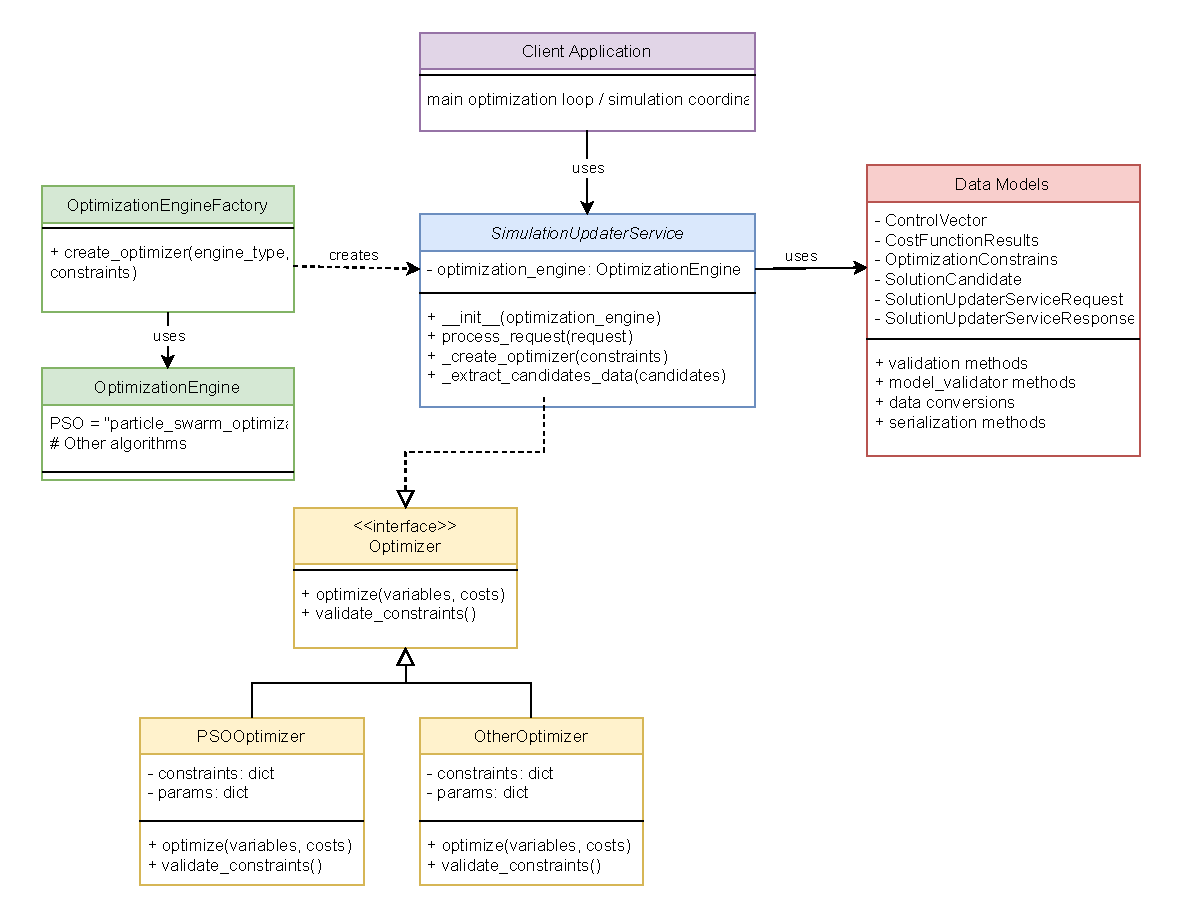
\includegraphics[width=1.0\textwidth]{content/images/SolutionUpdaterUML.pdf}
	\caption{Simulation updater service system UML}
	\label{fig:SolutionUpdaterServiceUML}
\end{figure}

\bigskip
\textbf{System Components}

The \texttt{SimulationUpdaterService} consists of several interconnected components that work together to provide optimization capabilities:

\begin{itemize}
\item \textbf{SimulationUpdaterService}

The main service class that exposes the public API and orchestrates the optimization process.

\textbf{Responsibilities:}
\begin{itemize}
	\item Provide a public interface for clients
	\item Coordinate the optimization workflow
	\item Manage the optimization loop
	\item Check convergence criteria
	\item Return processed results
\end{itemize}

\item \textbf{\_Mapper}

Internal component responsible for translating between domain-specific data structures and numerical representations suitable for optimization algorithms.

\textbf{Responsibilities:}
\begin{itemize}
	\item Convert control vectors to numpy arrays
	\item Convert optimization results back to domain objects
	\item Maintain mappings between domain and numerical representations
	\item Handle variable bounds and constraints
	\item Initialize mapping on first execution
\end{itemize}

\item \textbf{\_MapperState}

Maintains the state of mappings between control vectors, simulation results, and their numerical representations.

\textbf{Responsibilities:}
\begin{itemize}
	\item Store control vector mapping information
	\item Store results mapping information
	\item Track control vector dimensions
	\item Track results dimensions
	\item Store population size information
\end{itemize}

\item \textbf{\_SolutionUpdaterServiceLoopController}

Controls the execution of the optimization loop, tracking progress and termination conditions.

\textbf{Responsibilities:}
\begin{itemize}
	\item Track current generation number
	\item Enforce maximum generation limit
	\item Provide running state information
	\item Offer context manager for loop control
	\item Support early termination
\end{itemize}

\item \textbf{Optimization Engine}

Encapsulated component that implements the mathematical optimization algorithms.

\textbf{Responsibilities:}
\begin{itemize}
	\item Execute numerical optimization operations
	\item Apply optimization techniques to solution arrays
	\item Generate updated solutions based on fitness evaluations
	\item Handle constraints in the optimization process
\end{itemize}

\end{itemize}

\textbf{Public API}

The \texttt{SimulationUpdaterService} exposes a minimal yet powerful public API that provides access to its optimization capabilities. This section details each public method, its parameters, return values, and implementation details.

\begin{itemize}
	\item SimulationUpdaterService Constructor

	Initializes a new instance of the \texttt{SimulationUpdaterService} class. This constructor sets up the internal components required for the optimization process, including the mapper, optimization engine, and loop controller.

	\textbf{Implementation Details}

	The constructor performs the following initialization steps:
	\begin{itemize}
		\item Creates a new instance of the \texttt{\_Mapper} class for domain-numerical translation
		\item Initializes the optimization engine with default configuration
		\item Sets up a logger for diagnostic information
		\item Creates a \texttt{\_SolutionUpdaterServiceLoopController} instance to manage the optimization loop
	\end{itemize}

	\textbf{Error Handling}
	\begin{itemize}
		\item Any exceptions during initialization are allowed to propagate, as they indicate critical setup problems that should prevent service creation
		\item If dependencies are not available or incorrectly configured, appropriate import or initialization errors will be raised
	\end{itemize}

	\item \csignature{process\_request(self, request)}

	Processes an optimization request by iteratively updating the solution based on simulation results. This method represents the core functionality of the service, orchestrating the complete optimization workflow from initial population to converged solutions.

	\textbf{Implementation Details}

	The method implements a complete optimization step:
	\begin{enumerate}
		\item Validates the input request for required fields and data consistency
		\item Initializes the mapper with the domain-specific structure of control vectors and results
		\item Converts the domain objects to numerical arrays suitable for optimization
		\item Sets up the optimization loop with appropriate constraints and parameters
		\item Executes the optimization process for multiple generations until convergence or maximum generations
		\item Periodically checks for convergence based on defined criteria
		\item Translates the optimized numerical results back to domain-specific control vectors
		\item Prepares and returns a comprehensive response with the optimization results
	\end{enumerate}

	\textbf{Error Handling}
	\begin{itemize}
		\item \textbf{ValueError}: Raised if the request is missing required fields or contains inconsistent data
		\begin{itemize}
			\item Missing initial population or simulation results
			\item Mismatch between population size and results size
			\item Invalid configuration parameters (negative max generations, etc.)
		\end{itemize}

		\item \textbf{TypeError}: Raised if the data types in the request are incompatible with the optimization process
		\begin{itemize}
			\item Non-numeric values in control vectors or results
			\item Incompatible constraint formats
		\end{itemize}

		\item \textbf{RuntimeError}: Raised if the optimization process encounters an unrecoverable error
		\begin{itemize}
			\item Optimization algorithm failure
			\item Numerical stability issues
			\item Resource limitations
		\end{itemize}

		\item \textbf{Exception Handling}: The method includes comprehensive exception handling to:
		\begin{itemize}
			\item Log detailed diagnostic information
			\item Provide informative error messages
			\item Clean up resources in case of failures
			\item Convert low-level numerical exceptions to domain-appropriate exceptions
		\end{itemize}
	\end{itemize}

	\item \textbf{Loop controller}

	A property that provides access to the optimization loop controller. The loop controller exposes information about the optimization process state and provides control over the execution of the optimization loop:

	\begin{itemize}
		\item Maintains state about the current generation number
		\item Tracks whether the optimization loop is currently running
		\item Provides a context manager for the optimization loop execution
		\item Enforces maximum generation constraints
		\item Supports early termination of the optimization process
	\end{itemize}

	The controller is typically used internally by the \texttt{process\_request} method, but is exposed as a public property to allow advanced clients to access detailed state information or implement custom loop control if needed.

\end{itemize}

\textbf{Data Models Schema}

The \texttt{SimulationUpdaterService} uses a structured set of data models to represent optimization problems, solution candidates, and constraints. This section details the schemas of these models and their relationships.

\begin{lstlisting}[language=Python, caption={OptimizationEngine enumeration definition}]
	class OptimizationEngine(Enum):
	"""Enumeration of available optimization algorithms."""

	PSO = "particle_swarm_optimization"
	# Other algorithm types can be added here
\end{lstlisting}

\textbf{Description:}
The \texttt{OptimizationEngine} enumeration defines the available optimization algorithms that can be used by the service. Currently, it includes Particle Swarm Optimization (PSO), but the system is designed to be extensible with additional algorithms in the future.

\begin{lstlisting}[language=Python, caption={ControlVector model definition}]
	from pydantic import BaseModel, Field

	class ControlVector(BaseModel, extra="forbid"):
	"""Represents a collection of optimization variables."""

	items: Dict[str, float]
\end{lstlisting}

\textbf{Description:}
The \texttt{ControlVector} model represents the input parameters that control a simulation. Each item in the dictionary corresponds to a single optimization variable (e.g., "pressure", "temperature") with its associated value. The optimization process will aim to find optimal values for these variables.

\textbf{Validation Requirements:}
\begin{itemize}
	\item The items dictionary must not be empty
	\item All keys must be strings representing variable names
	\item All values must be floating-point numbers within valid numerical ranges
\end{itemize}

\begin{lstlisting}[language=Python, caption={CostFunctionResults model definition}]
	from pydantic import BaseModel, Field

	class CostFunctionResults(BaseModel, extra="forbid"):
	"""Stores the results of cost function calculations."""

	values: Dict[str, float]
\end{lstlisting}

\textbf{Description:}
The \texttt{CostFunctionResults} model stores the output metrics from simulation runs. Each item in the dictionary represents a cost function (e.g., "heat\_transfer", "flow\_rate") with its calculated value. These values are used to evaluate how good a particular solution is and guide the optimization process.

\textbf{Validation Requirements:}
\begin{itemize}
	\item The values dictionary must not be empty
	\item All keys must be strings representing cost function names
	\item All values must be floating-point numbers
\end{itemize}

\begin{lstlisting}[language=Python, caption={OptimizationConstrains model with validation logic}]
	from pydantic import BaseModel, Field, model_validator

	class OptimizationConstrains(BaseModel, extra="forbid"):
	"""Defines the constraints for the optimization variables."""

	boundaries: Dict[str, Tuple[float, float]]

	@model_validator(mode='after')
	def validate_lower_bound_is_less_than_upper_bound(self) -> 'OptimizationConstrains':
	"""Validates that lower bounds are less than upper bounds."""
		for var_name, (lower, upper) in self.boundaries.items():
			if lower >= upper:
				raise ValueError(
				f"Lower bound must be less than upper bound for {var_name}. "
				f"Got: lower={lower}, upper={upper}"
		)
	return self
\end{lstlisting}


\textbf{Description:}
The \texttt{OptimizationConstrains} model defines the valid ranges for optimization variables. Each entry in the boundaries dictionary maps a variable name to its allowed range as a tuple of (lower\_bound, upper\_bound). The optimization process will ensure that all solutions stay within these boundaries.

\textbf{Validation Requirements:}
\begin{itemize}
	\item For each variable, the lower bound must be strictly less than the upper bound
	\item All boundary values must be valid floating-point numbers
	\item Variable names in boundaries should match those used in ControlVector
\end{itemize}

\begin{lstlisting}[language=Python, caption={SolutionCandidate model definition}]
	from pydantic import BaseModel, Field

	class SolutionCandidate(BaseModel, extra="forbid"):
	"""Represents a complete solution with inputs and results."""

	control_vector: ControlVector
	cost_function_results: CostFunctionResults
\end{lstlisting}

\textbf{Description:}
The \texttt{SolutionCandidate} model represents a complete solution in the optimization process, pairing a specific set of input parameters with their resulting simulation outputs. Each candidate represents one point in the solution space, and the optimization process evaluates and compares candidates to find better solutions.

\textbf{Validation Requirements:}
\begin{itemize}
	\item Both control\_vector and cost\_function\_results must be provided
	\item The control\_vector must be a valid ControlVector instance
	\item The cost\_function\_results must be a valid CostFunctionResults instance
\end{itemize}

\begin{lstlisting}[language=Python, caption={SolutionUpdaterServiceRequest model with complex validation logic}]
	from pydantic import BaseModel, Field, model_validator
	from typing import List, Optional

	class SolutionUpdaterServiceRequest(BaseModel, extra="forbid"):
	"""The complete request for optimization."""

	solution_candidates: List[SolutionCandidate]
	optimization_constraints: Optional[OptimizationConstrains] = None

	@model_validator(mode='after')
	def validate_solution_candidates_contain_the_same_cost_functions(self) -> 'SolutionUpdaterServiceRequest':
	"""Validates that all solution candidates use the same set of cost functions."""
	if not self.solution_candidates:
	return self

	reference_candidate = self.solution_candidates[0]
	reference_cost_functions = set(reference_candidate.cost_function_results.values.keys())

	for idx, candidate in enumerate(self.solution_candidates[1:], start=1):
	candidate_cost_functions = set(candidate.cost_function_results.values.keys())
	if reference_cost_functions != candidate_cost_functions:
	raise ValueError(
	f"All solution candidates must contain the same cost functions. "
	f"Mismatch at candidate {idx}. "
	f"Expected: {reference_cost_functions}, "
	f"Got: {candidate_cost_functions}"
	)
	return self

	@model_validator(mode='after')
	def validate_solution_candidates_contain_the_same_optimization_variables(self) -> 'SolutionUpdaterServiceRequest':
	"""Validates that all solution candidates use the same set of optimization variables."""
	if not self.solution_candidates:
	return self

	reference_candidate = self.solution_candidates[0]
	reference_variables = set(reference_candidate.control_vector.items.keys())

	for idx, candidate in enumerate(self.solution_candidates[1:], start=1):
	candidate_variables = set(candidate.control_vector.items.keys())
	if reference_variables != candidate_variables:
	raise ValueError(
	f"All solution candidates must contain the same optimization variables. "
	f"Mismatch at candidate {idx}. "
	f"Expected: {reference_variables}, "
	f"Got: {candidate_variables}"
	)
	return self

	@model_validator(mode='after')
	def validate_optimization_boundaries_contain_the_same_optimization_variables(self) -> 'SolutionUpdaterServiceRequest':
	"""Validates that optimization boundaries match the variables used in solutions."""
	if not self.solution_candidates or not self.optimization_constraints:
	return self

	reference_candidate = self.solution_candidates[0]
	reference_variables = set(reference_candidate.control_vector.items.keys())
	boundary_variables = set(self.optimization_constraints.boundaries.keys())

	if reference_variables != boundary_variables:
	raise ValueError(
	f"Optimization boundaries must contain the same variables as solution candidates. "
	f"Solution variables: {reference_variables}, "
	f"Boundary variables: {boundary_variables}"
	)
	return self

	@model_validator(mode='after')
	def reorder_solution_candidates_optimization_variables_and_cost_functions(self) -> 'SolutionUpdaterServiceRequest':
	"""Reorders variables and cost functions for consistent processing."""
	# Implementation handles consistency of ordering across solution candidates
	return self
\end{lstlisting}

\textbf{Description:}
The \texttt{SolutionUpdaterServiceRequest} model represents a complete request to the optimization service. It contains the initial population of solution candidates and optional constraints. The service processes this request to generate an optimized set of solutions.

The model includes several validation methods to ensure consistency across the solution candidates:
\begin{itemize}
	\item Ensures all candidates use the same cost functions
	\item Ensures all candidates use the same optimization variables
	\item Verifies that optimization boundaries match the variables used
	\item Reorders variables and cost functions for consistent processing
\end{itemize}

\textbf{Validation Requirements:}
\begin{itemize}
	\item Must contain at least one solution candidate
	\item All solution candidates must use the same set of cost function names
	\item All solution candidates must use the same set of optimization variable names
	\item If constraints are provided, they must cover the same variable names
\end{itemize}







\bigskip
\textbf{Detailed Workflow}
The optimization process within the \texttt{SimulationUpdaterService} follows a systematic workflow that translates domain-specific inputs into optimized outputs through several processing stages.

\begin{enumerate}

\item Initialization Phase

\begin{enumerate}
	\item \textbf{Request Validation}: The service validates the incoming request to ensure it contains the required data.

	\item \textbf{Mapper Initialization}: On first execution, the mapper analyzes the structure of control vectors and results to create appropriate mappings.

	\item \textbf{State Preparation}: The service initializes the optimization state, including:
	\begin{itemize}
		\item Population arrays
		\item Results arrays
		\item Constraint definitions
		\item Variable bounds
		\item Generation counters
	\end{itemize}

	\item \textbf{Engine Configuration}: The optimization engine is configured with appropriate parameters for the specific problem.
\end{enumerate}

\item Optimization Step

The main optimization step executes the following steps for each generation:

\begin{enumerate}
	\item \textbf{Population Conversion}: Control vectors are converted to numerical arrays using the mapper.

	\item \textbf{Fitness Evaluation}: The fitness of each solution is calculated based on simulation results.

	\item \textbf{Selection}: The most promising individuals are selected for producing the next generation.

	\item \textbf{Variation Operations}: The optimization engine applies:
	\begin{itemize}
		\item Crossover between selected individuals
		\item Mutation to maintain diversity
		\item Constraint handling to ensure valid solutions
	\end{itemize}

	\item \textbf{Population Update}: The new generation replaces the previous one.

	\item \textbf{Convergence Check}: The service evaluates whether the optimization has converged using:
	\begin{itemize}
		\item Change in objective function values
		\item Population diversity metrics
		\item Constraint satisfaction levels
		\item Stability of the best solution
	\end{itemize}

	\item \textbf{Loop Control}: The controller updates generation counters and checks for termination conditions.
\end{enumerate}

\item Finalization Phase

After the optimization step completes (either through convergence or reaching maximum generations):

\begin{enumerate}
	\item \textbf{Result Translation}: The final numerical solutions are converted back to domain-specific control vectors.

	\item \textbf{Metrics Compilation}: Convergence metrics and optimization statistics are compiled.

	\item \textbf{Response Preparation}: A structured response is created containing:
	\begin{itemize}
		\item Optimized control vectors
		\item Convergence metrics and history
		\item Termination reason
		\item Generation statistics
	\end{itemize}

	\item \textbf{Resource Cleanup}: Any temporary resources used during optimization are released.
\end{enumerate}

\end{enumerate}

\subsubsection{Problem dispatcher service}

\subsection{Orchestration}
\label{sec:orchestration}

\subsection{Data flow}
\label{sec:data-flow}

\subsection{Orchestration}
\label{sec:orchestration}


	\section{Services}

\subsection{Well management service}

\subsubsection{Overview}

The \texttt{WellManagementService} is a service component responsible for handling well configuration requests and building appropriate well models for simulation. It processes requests containing well specifications, constructs wells based on various templates (I-well, J-well, S-well, H-well), and returns a response with simulation-ready well models.

\subsubsection{Architecture}

The well management subsystem follows a layered architecture with clear separation of concerns.

\begin{itemize}
	\item \texttt{WellManagementService}
	\item \texttt{WellTemplateInterface} (Abstract)
	\begin{itemize}
		\item \texttt{IWellTemplate} (Vertical well)
		\item \texttt{JWellTemplate} (J-shaped well)
		\item \texttt{SWellTemplate} (S-shaped well)
		\item \texttt{HWellTemplate} (Horizontal well)
	\end{itemize}
	\item \texttt{SectionInterface} (Abstract)
	\begin{itemize}
		\item \texttt{LinearWellSection}
		\item \texttt{CurvedWellSection}
	\end{itemize}
	\item \texttt{WellBuilder}
	\item Support classes:
	\begin{itemize}
		\item \texttt{PerforationMdProvider}
		\item \texttt{PerforationRange}
	\end{itemize}
\end{itemize}

This architecture provides several benefits:
\begin{itemize}
	\item \textbf{Separation of Concerns}: Each component has a specific, focused responsibility.
	\item \textbf{Extensibility}: New well types can be added by creating new templates without modifying existing code.
	\item \textbf{Maintainability}: The builder pattern isolates construction logic, making it easier to update.
	\item \textbf{Testability}: Components can be tested in isolation with appropriate mocks.
\end{itemize}

\begin{figure}[H]
	\centering
	\includesvg[width=1.0\textwidth]{content/images/WellManagementServiceUML}
	\caption{Well management service system UML}
	\label{fig:WellManagementServiceUML}
\end{figure}


\subsubsection{System components}
\begin{itemize}
	\item \textbf{WellManagementService}: Acts as a facade for the subsystem, receiving JSON requests, coordinating the creation of wells, and returning standardized responses.

	\item \textbf{Well Templates}: Specialized factories for different well types (I-well, J-well, S-well, H-well) that encapsulate the configuration logic specific to each well geometry.

	\item \textbf{WellBuilder}: Implements the builder pattern to provide a fluent interface for constructing complex well objects with various configurations.

	\item \textbf{Well Models}: Data structures representing wells and their properties, used both for input configuration and output results.
\end{itemize}

The flow of data through the system is as follows:

\begin{enumerate}
	\item Client sends a request with well configurations to the WellManagementService.
	\item The service parses the request and identifies the well types needed.
	\item For each well configuration, the appropriate template is selected and used.
	\item Templates configure WellBuilder instances with the correct geometrical properties.
	\item WellBuilder constructs complete Well objects with the specified properties.
	\item Wells are converted to SimulationWellModels for the response.
	\item The service returns a standardized response with the constructed wells.
\end{enumerate}


\subsubsection{Public API}

	\begin{verbatim}
		process_request(request_dict: dict[str, Any]) -> WellManagementServiceResponse
	\end{verbatim}

Main entry point for the service. Processes a dictionary representation of a well management request.

\begin{itemize}
	\item \textbf{Parameters:}
	\begin{itemize}
		\item \texttt{request\_dict}: Dictionary containing well specification data
	\end{itemize}
	\item \textbf{Returns:}
	\begin{itemize}
		\item \texttt{WellManagementServiceResponse}: Object containing processed simulation well models
	\end{itemize}
	\item \textbf{Description:}\\
	This method parses the input dictionary into a \texttt{WellManagementServiceRequest} object, logs the parsed request for debugging purposes, and delegates to the private \texttt{\_build\_wells} method to generate the wells based on the request configuration. The final result is a \texttt{WellManagementServiceResponse} containing simulation-ready well models.
\end{itemize}

\begin{verbatim}
dump_results_schema(path: Path | str) -> None
\end{verbatim}


Generates and saves the JSON schema for the service response.

\begin{itemize}
\item \textbf{Parameters:}
\begin{itemize}
\item \texttt{path}: File path (as string or Path object) where the schema will be saved
\end{itemize}
\item \textbf{Returns:}
\begin{itemize}
\item None
\end{itemize}
\item \textbf{Description:}\\
This method generates the JSON schema for the \texttt{WellManagementServiceResponse} class and writes it to the specified path. This schema documentation can be used by clients to understand the structure of the service response.
\end{itemize}



\subsubsection{Data Models Schema}

\textbf{PerforationRangeModel}
\begin{figure}[H]
	\begin{lstlisting}[language=Python, caption=PerforationRangeModel class definition]
		class PerforationRangeModel(BaseModel):
		start_md: float
		end_md: float
	\end{lstlisting}
\end{figure}

Defines a perforation range in measured depth along a wellbore.

\begin{itemize}
	\item \textbf{Attributes:}
	\begin{itemize}
		\item \texttt{start\_md}: Starting measured depth of the perforation
		\item \texttt{end\_md}: Ending measured depth of the perforation
	\end{itemize}
	\item \textbf{Validation:}
	\begin{itemize}
		\item Ensures that \texttt{start\_md} is less than \texttt{end\_md}
	\end{itemize}
\end{itemize}

\textbf{PositionModel}
\begin{figure}[H]
	\begin{lstlisting}[language=Python, caption=PositionModel class definition]
		class PositionModel(BaseModel):
		x: float
		y: float
		z: float
	\end{lstlisting}
\end{figure}

Represents a 3D coordinate position.

\begin{itemize}
	\item \textbf{Attributes:}
	\begin{itemize}
		\item \texttt{x}: X-coordinate
		\item \texttt{y}: Y-coordinate
		\item \texttt{z}: Z-coordinate
	\end{itemize}
\end{itemize}

\textbf{IWellModel}
\begin{figure}[H]
	\begin{lstlisting}[language=Python, caption=IWellModel class definition]
		class IWellModel(BaseModel):
		well_type: Literal["I"] = "I"
		name: str
		md: float
		wellhead: tuple[float, float, float]
		md_step: float = Field(ge=0.1)
		perforations: list[PerforationRangeModel] = []
	\end{lstlisting}
\end{figure}

Represents a vertical (I-type) well.

\begin{itemize}
	\item \textbf{Attributes:}
	\begin{itemize}
		\item \texttt{well\_type}: Fixed as "I" to identify the well type
		\item \texttt{name}: Name of the well
		\item \texttt{md}: Maximum measured depth (total length) of the well
		\item \texttt{wellhead}: 3D coordinates of the wellhead (starting point)
		\item \texttt{md\_step}: Discretization step size along the well (must be greater than or equal to 0.1)
		\item \texttt{perforations}: List of perforation ranges along the well (default: empty list)
	\end{itemize}
\end{itemize}

\textbf{JWellModel}
\begin{figure}[H]
	\begin{lstlisting}[language=Python, caption=JWellModel class definition]
		class JWellModel(BaseModel):
		well_type: Literal["J"] = "J"
		name: str
		md_linear1: float
		md_curved: float
		dls: float
		md_linear2: float
		wellhead: tuple[float, float, float]
		azimuth: float = 0.0
		md_step: float = Field(ge=0.1)
		perforations: list[PerforationRangeModel] = []
	\end{lstlisting}
\end{figure}

Represents a J-shaped well with one curved section.

\begin{itemize}
	\item \textbf{Attributes:}
	\begin{itemize}
		\item \texttt{well\_type}: Fixed as "J" to identify the well type
		\item \texttt{name}: Name of the well
		\item \texttt{md\_linear1}: Measured depth of the first (vertical) linear section
		\item \texttt{md\_curved}: Measured depth of the curved section
		\item \texttt{dls}: Dogleg severity (rate of change in angle) in degrees per unit length
		\item \texttt{md\_linear2}: Measured depth of the second (deviated) linear section
		\item \texttt{wellhead}: 3D coordinates of the wellhead (starting point)
		\item \texttt{azimuth}: Azimuth angle in degrees (default: 0.0)
		\item \texttt{md\_step}: Discretization step size along the well (must be greater than or equal to 0.1)
		\item \texttt{perforations}: List of perforation ranges along the well (default: empty list)
	\end{itemize}
\end{itemize}

\textbf{SWellModel}
\begin{figure}[H]
	\begin{lstlisting}[language=Python, caption=SWellModel class definition]
		class SWellModel(BaseModel):
		well_type: Literal["S"] = "S"
		name: str
		md_linear1: float
		md_curved1: float
		dls1: float
		md_linear2: float
		md_curved2: float
		dls2: float
		md_linear3: float
		wellhead: tuple[float, float, float]
		azimuth: float = 0.0
		md_step: float = Field(ge=0.1)
		perforations: list[PerforationRangeModel] = []
	\end{lstlisting}
\end{figure}

Represents an S-shaped well with two curved sections.

\begin{itemize}
	\item \textbf{Attributes:}
	\begin{itemize}
		\item \texttt{well\_type}: Fixed as "S" to identify the well type
		\item \texttt{name}: Name of the well
		\item \texttt{md\_linear1}: Measured depth of the first (vertical) linear section
		\item \texttt{md\_curved1}: Measured depth of the first curved section
		\item \texttt{dls1}: Dogleg severity for the first curved section in degrees per unit length
		\item \texttt{md\_linear2}: Measured depth of the second (intermediate) linear section
		\item \texttt{md\_curved2}: Measured depth of the second curved section
		\item \texttt{dls2}: Dogleg severity for the second curved section in degrees per unit length
		\item \texttt{md\_linear3}: Measured depth of the third (final) linear section
		\item \texttt{wellhead}: 3D coordinates of the wellhead (starting point)
		\item \texttt{azimuth}: Azimuth angle in degrees (default: 0.0)
		\item \texttt{md\_step}: Discretization step size along the well (must be greater than or equal to 0.1)
		\item \texttt{perforations}: List of perforation ranges along the well (default: empty list)
	\end{itemize}
\end{itemize}

\textbf{HWellModel}
\begin{figure}[H]
	\begin{lstlisting}[language=Python, caption=HWellModel class definition]
		class HWellModel(BaseModel):
		well_type: Literal["H"] = "H"
		name: str
		TVD: float
		md_lateral: float
		wellhead: tuple[float, float, float]
		azimuth: float = 0.0
		md_step: float = Field(ge=0.1)
		perforations: list[PerforationRangeModel] = []
	\end{lstlisting}
\end{figure}

Represents a horizontal well with a vertical section followed by a lateral section.

\begin{itemize}
	\item \textbf{Attributes:}
	\begin{itemize}
		\item \texttt{well\_type}: Fixed as "H" to identify the well type
		\item \texttt{name}: Name of the well
		\item \texttt{TVD}: True vertical depth (vertical section length)
		\item \texttt{md\_lateral}: Measured depth of the lateral (horizontal) section
		\item \texttt{wellhead}: 3D coordinates of the wellhead (starting point)
		\item \texttt{azimuth}: Azimuth angle in degrees (default: 0.0)
		\item \texttt{md\_step}: Discretization step size along the well (must be greater than or equal to 0.1)
		\item \texttt{perforations}: List of perforation ranges along the well (default: empty list)
	\end{itemize}
\end{itemize}

\textbf{WellManagementServiceRequest}
\begin{figure}[H]
	\begin{lstlisting}[language=Python, caption=WellManagementServiceRequest class definition]
		class WellManagementServiceRequest(BaseModel):
		models: list[IWellModel | JWellModel | SWellModel | HWellModel]
	\end{lstlisting}
\end{figure}

Represents a request to the well management service.

\begin{itemize}
	\item \textbf{Attributes:}
	\begin{itemize}
		\item \texttt{models}: List of well models to be processed
	\end{itemize}
\end{itemize}

\textbf{SimulationWellPerforationModel}
\begin{figure}[H]
	\begin{lstlisting}[language=Python, caption=SimulationWellPerforationModel class definition]
		class SimulationWellPerforationModel(BaseModel):
		range: tuple[float, float]
	\end{lstlisting}
\end{figure}

Represents a perforation range in a simulation well model.

\begin{itemize}
	\item \textbf{Attributes:}
	\begin{itemize}
		\item \texttt{range}: Tuple containing the start and end measured depths of the perforation
	\end{itemize}
\end{itemize}

\textbf{WellManagementServiceResponse}
\begin{figure}[H]
	\begin{lstlisting}[language=Python, caption=WellManagementServiceResponse class definition]
		class WellManagementServiceResponse(BaseModel):
		wells: list[SimulationWellModel]
	\end{lstlisting}
\end{figure}

Represents a response from the well management service.

\begin{itemize}
	\item \textbf{Attributes:}
	\begin{itemize}
		\item \texttt{wells}: List of simulation well models generated from the request
	\end{itemize}
\end{itemize}

\subsubsection{Shared models}

Service do not use any shared data models.

\subsubsection{Detailed Workflow}

The \texttt{WellManagementService} provides a comprehensive framework for building and managing various types of well models in petroleum engineering applications. It offers a flexible architecture for creating wells with different geometries including vertical (I-shaped), J-shaped, S-shaped, and horizontal (H-shaped) wells.

The service follows a clear workflow for processing well creation requests:

\begin{enumerate}
	\item Client submits a request containing well specifications
	\item \texttt{WellManagementService.process\_request()} parses the request into a \texttt{WellManagementServiceRequest} object
	\item Service identifies well model types in the request (I, J, S, or H)
	\item For each model, the appropriate template is instantiated
	\item Each template configures and uses a \texttt{WellBuilder} to construct the well
	\item All constructed wells are collected and returned in a \texttt{WellManagementServiceResponse}
\end{enumerate}

The \texttt{WellManagementService} provides a flexible and extensible framework for building various types of well models with different geometries and completions. The architecture leverages design patterns such as Template Method, Builder, and Strategy to create a maintainable and scalable system.


\subsubsection{Dependencies}

\subsubsection{Well models}

	The well model is located in the xz plane as shown on the picture below (note that the z-axis is defined upside down). The LinearWellSection is s fragment of a straight line. Inclination $(\theta)$ is defined as an angle between z-axis and the section. Its values can vary from $-180\degree$ to $180\degree$.

	\begin{figure}[H]
		\centering
		\includegraphics[scale=0.6]{images/well_builder/linear\_section.png}
		\caption{Illustrative drawing of the linear section.}
		\label{linear_section}
	\end{figure}

	The section always starts at the last point in the trajectory (here the coordinate system is centered at that point). If $\theta$ is not provided it is calculated from coordinates of last two points form the trajectory as, such that the section is parallel to the line spanned by these points:
	\begin{equation}
		\theta = \mathrm{atan}\left(\frac{x_{-1} - x_{-2}}{z_{-1} - z_{-2}}\right)
	\end{equation}
	If $z_{-1} - z_{-2} >= 0$, and:
	\begin{equation}
		\theta = \pi + \mathrm{atan}\left(\frac{x_{-1} - x_{-2}}{z_{-1} - z_{-2}}\right)
	\end{equation}
	If the results turns out to be outside of $[-180\degree, 180\degree]$ it needs to be rotated by $-360\degree$.
	\begin{itemize}
		\item $(x_{-1}, z_{-1})$ - coordinates of the last point
		\item $(x_{-2}, z_{-2})$ - coordinates of the second last point
	\end{itemize}

	The curved section is an arc of a circle. It is more complicated than the linear section as in general there are 8 cases. On the picture below the curved sections are shown as starting at the ends of linear sections which are in the trajectory before them. The linear section starting at point (0, 0) is located in one of four quadrants of the coordinate system. In each of these cases the curved segment can curve in 2 directions (clockwise or counter-clockwise). All the cases are shown on the picture below.
	\begin{figure}[H]
		\centering
		\includegraphics[scale=0.4]{images/well_builder/curved\_section.png}
		\caption{Illustrative drawing of the curved section cases.}
		\label{curved_section}
	\end{figure}
	\begin{itemize}
		\item red rods - start points of the curved sections
		\item blue dots - centers of the circles
		\item $\theta$ - inclination
		\item arrows - show direction of curvature
		\item sign of $dls$ encodes information if the start point of the section is on the lower or the upper part of the circle.\\
		$dls > 0$ - start point is on the lower part\\
		$dls < 0$ - start point is on the upper part\\
	\end{itemize}
	In this case inclination is interpreted as the angle between z-axis and the straight line tangent to the trajectory at the start point. If not given it is calculated the same way as it was described in the LinearWellSection. Absolute value of dls is the angle change in degrees over 30 meters of measured distance.\newline

	To determine the trajectory several quantities need to be calculated. These are:
	\begin{itemize}
		\item Circle radius
		\item Angle increase - absolute value of the angular coordinate change in polar coordinates centered on the circle center
		\item Circle center location
		\item Starting point - angular coordinate in polar coordinates centered on the circle center
	\end{itemize}
	Radius is calculated as:
	\begin{equation}
		R = \left|\frac{30} {dls}\right|
	\end{equation}
	where $dls$ is given in radians.\newline
	Angle increase is calculated as:
	\begin{equation}
		\Delta \phi = \frac{md}{R}
	\end{equation}
	Circle center's location is calculated as:
	\begin{equation}
		x_0 = x + sign_x \cdot R \cdot \mathrm{cos}(\theta)
	\end{equation}
	\begin{equation}
		z_0 = z + sign_z \cdot R \cdot \mathrm{sin}(\theta)
	\end{equation}
	\begin{itemize}
		\item $(x_0, z_0)$ - location of the center
		\item $(x, z)$ - location of the starting point
	\end{itemize}
	$sign_x$ and $sign_z$ values are determined by the particular case:

	\begin{itemize}
		\item $sign_x$ = 1 if ($dls >=0$ and $\alpha >= 0$) or ($dls < 0$ and $\alpha < 0$), = -1 otherwise
		\item $sign_z$ = -1 if ($dls >= 0$), = 1 otherwise
	\end{itemize}


	To calculate the angular location of the starting point we introduce parameters:
	\begin{itemize}
		\item $r_x = x - x_0$
		\item $r_z = z - z_0$
	\end{itemize}
	They cannot both be zero as it would mean that the center is in the wellbore.\newline
	The boundary case is $rx=0$. It appears when $\theta = \frac{\pi}{2}$ or $\theta = -\frac{\pi}{2}$. It has subcases:
	\begin{itemize}
		\item $r_x=0$, $r_z<0$: $\phi_{start} = \frac{\pi}{2}$
		\item $r_x=0$, $r_z>0$, $\theta>=0$: $\phi_{start} = -\frac{\pi}{2}$
		\item $r_x=0$, $r_z>0$, $\theta>=0$: $\phi_{start} = \frac{3\pi}{2}$
	\end{itemize}
	$-\frac{\pi}{2}$ and $\frac{3\pi}{2}$ are technically equal. They are treated here separately for computational convenience. To the first one angle increase will be added and from the second one substracted.\newline
	Now we will consider the rest of the cases:
	\begin{itemize}
		\item $r_x>0$, $r_z>0$: $\phi_{start} = -\mathrm{atan}\left(\frac{r_z}{r_x}\right)$
		\item $r_x<0$, $r_z<0$: $\phi_{start} = \pi-\mathrm{atan}\left(\frac{r_z}{r_x}\right)$
		\item $r_x>0$, $r_z<0$: $\phi_{start} = \mathrm{atan}\left(\frac{r_z}{r_x}\right)$
		\item $r_x<0$, $r_z>0$: $\phi_{start} = \pi + \mathrm{atan}\left(\frac{r_z}{r_x}\right)$
	\end{itemize}

	Relation between inclination, dls and curvature direction was presented on the following figure:\\\\
	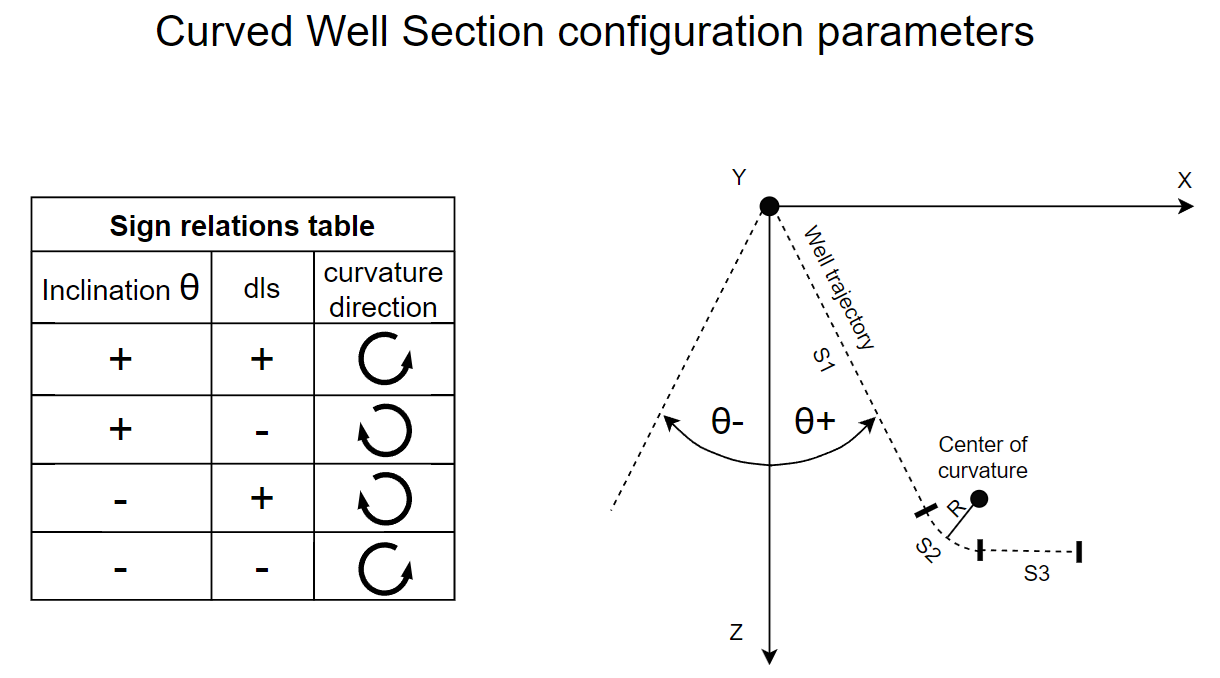
\includegraphics[width=1.0\textwidth]{"images/well_builder/dls_vs_inclination.png"}

\subsubsection{Simulation service}
\textbf{Overview}

\texttt{SimulationService} is a high-performance distributed simulation management system designed to orchestrate, execute, and monitor simulation tasks across a computational cluster. The service provides a robust API for transferring simulation models, processing requests, and managing the lifecycle of the simulation infrastructure.

\bigskip
\textbf{Architecture}

The service is built on a client-server architecture using gRPC for high-performance communication. It leverages a worker pool pattern to distribute simulation workloads efficiently across available computational resources. \texttt{SimulationService} system architecture is present in Fig. \ref{fig:SimulationServiceSystemArchitecture}.

\bigskip
\textbf{System Components}

\bigskip
Main system components:

\begin{itemize}
	\item \textbf{Simulation Service} - main service class, where user or optimization system reach simulation cluster

	\item \textbf{Server} - Central coordinator of the simulation cluster, build from dedicated \textit{Dockerfile}. Launched as \textit{Docker container} via \textit{Docker compose}. Communication between \textbf{Simulation Service} and \textbf{Worker(s)} are handled using gRPC protocol.

	Responsibilities:
	\begin{itemize}
		\item Accepts simulation model uploads
		\item Distributes simulation jobs to available workers
		\item Tracks simulation progress and collects results
		\item Maintains state about connected workers and available models
	\end{itemize}

	\item \textbf{Worker Pool} - Compute nodes responsible for executing simulation jobs. Built from a \textit{Dockerfile}. Can be replicated (N instances) to scale horizontally. Initialized on cluster start and shut down on cluster termination.
		Responsibilities:
	\begin{itemize}
		\item Connect to the server and introduce themselves.
		\item Retrieve the simulation model from the server.
		\item Poll for simulation jobs.
		\item Perform simulations using the provided model and case data.
		\item Return simulation results to the server.
	\end{itemize}

\end{itemize}

% \begin{figure}[H]
% 	\centering
% 	\includesvg[width=1.0\textwidth]{content/images/SimulationServiceArchitecture}
% 	\caption{Simulation service system architecture}
% 	\label{fig:SimulationServiceSystemArchitecture}
% \end{figure}

\begin{figure}[H]
	\centering
	\includesvg[width=1.0\textwidth]{content/images/SimulationServiceUML}
	\caption{Simulation service system UML}
	\label{fig:SimulationServiceUML}
\end{figure}

\textbf{Public API}
\begin{itemize}
	\item \textbf{Cluster Management}

	 \csignature{\textit{start\_simulation\_cluster() $\rightarrow$ None}}

	 Initializes and launches the simulation cluster with the configured number of worker processes.

	 \textbf{Implementation Details:}
	 \begin{itemize}
	 	\item Validates environment configuration
	 	\item Starts the gRPC server on the configured host and port
	 	\item Initializes the worker pool with \texttt{\_WORKER\_COUNT} workers
	 	\item Establishes communication channels between server and workers
	 	\item Performs health checks to ensure cluster readiness
	 \end{itemize}

	 \textbf{Thread Safety:} Thread-safe, but should not be called concurrently with \texttt{shutdown\_simulation\_cluster()}

	 \textbf{Error Handling:} Raises exceptions for configuration issues, network failures, or resource allocation problems

	\csignature{\textit{shutdown\_simulation\_cluster() $\rightarrow$ None}}

	Safely terminates the simulation cluster and releases all resources.
	\textbf{Implementation Details:}
	\begin{itemize}
		\item Gracefully shuts down active simulation tasks
		\item Releases worker processes
		\item Closes network connections
		\item Cleans up temporary files and resources
	\end{itemize}

	\textbf{Thread Safety:} Thread-safe, but should not be called concurrently with \texttt{start\_simulation\_cluster()}

	\textbf{Error Handling:} Logs errors during shutdown but attempts to complete the process regardless of failures

	\item \textbf{Simulation Execution}

	\csignature{\textit{process\_request(request)}}

	Processes a simulation request by distributing tasks to the worker pool and aggregating results.

	\textbf{Parameters:}
	\begin{itemize}
		\item \texttt{request}: A simulation request object containing parameters and configuration for the simulation
	\end{itemize}

	\textbf{Returns:}
	\begin{itemize}
		\item Processed simulation results based on the request type
	\end{itemize}

	\textbf{Implementation Details:}
	\begin{itemize}
		\item Validates and normalizes the request
		\item Determines optimal task distribution strategy
		\item Distributes tasks to worker processes
		\item Monitors execution and handles failures
		\item Aggregates and post-processes results
	\end{itemize}

	\textbf{Thread Safety:} Thread-safe, can be called concurrently

	\textbf{Error Handling:} Returns error details for invalid requests, worker failures, or timeout issues

	\item \textbf{Model Management}

	\csignature{transfer\_simulation\_model(model)}

	Prepares and transfers a simulation model to all worker nodes in the cluster via simulation server.

	\textbf{Parameters:}
	\begin{itemize}
		\item \texttt{model}: The simulation model to distribute to the cluster
	\end{itemize}

	\textbf{Implementation Details:}
	\begin{itemize}
		\item Serializes the model into an appropriate format
		\item Compresses and optimizes the model for network transfer
		\item Distributes the model to all workers in the cluster
		\item Verifies successful model installation on each worker
	\end{itemize}

	\textbf{Thread Safety:} Thread-safe, but performance may degrade with concurrent transfers

	\textbf{Error Handling:} Raises exceptions for serialization failures, network issues, or worker-side installation problems

\end{itemize}

\textbf{Data Models Schema}

The \texttt{SimulationService} uses a well-defined set of data models for handling simulation requests, cases, and results. Understanding these models is essential for effectively using the service.

\begin{figure}[H]
	\begin{lstlisting}[language=Python, caption={SimulationResults Model}]
		class SimulationResults(BaseModel):
		"""
		Container for simulation calculation results.

		Contains heat results that may be represented in various formats:
		- Single value
		- Sequence of values
		- Matrix (sequence of sequences)

		Note: This implementation aligns with SimulationResultType
		and SimulationResults from common.py
		"""
		Heat: float | Sequence[float] | Sequence[Sequence[float] | float]
	\end{lstlisting}
\end{figure}

\begin{figure}[H]
	\begin{lstlisting}[language=Python, caption={SimulationCase Model}]
		class SimulationCase(BaseModel):
		"""
		Represents a single simulation case with inputs and optional results.

		Attributes:
		wells: Well configuration data from the WellManagement service
		control_vector: Dictionary mapping control parameters to their values
		results: Optional field containing simulation results when completed
		"""
		wells: WellManagementServiceResult
		control_vector: dict[str, float]
		results: SimulationResults | None = Field(default=None)
	\end{lstlisting}
\end{figure}

\begin{figure}[H]
	\begin{lstlisting}[language=Python, caption={SimulationServiceRequest Model}]
		class SimulationServiceRequest(BaseModel):
		"""
		Container for a batch of simulation cases to be processed.

		Attributes:
		simulation_cases: List of simulation cases to be executed
		"""
		simulation_cases: list[SimulationCase]
	\end{lstlisting}
\end{figure}

\begin{figure}[h]
	\begin{lstlisting}[language=Python, caption={SimulationServiceResponse Model}]
		class SimulationServiceResponse(BaseModel):
		"""
		Container for processed simulation cases with results.

		Attributes:
		simulation_cases: List of simulation cases with populated results
		"""
		simulation_cases: list[SimulationCase]
	\end{lstlisting}
\end{figure}

\textbf{Shared models:}
\begin{enumerate}
	\item Well Management Service Models

	The SimulationService integrates with the Well Management Service through a set of shared models that define well configurations, trajectories, and completions. These models provide the foundation for simulation cases.

	\begin{figure}[H]
		\begin{lstlisting}[language=Python, caption={SimulationWellPerforation Model}]
			class SimulationWellPerforationModel(BaseModel):
			"""
			Represents a perforation in a well with a depth range and 3D coordinate points.

			Attributes:
			range: Tuple defining the start and end depths of the perforation
			points: Collection of 3D points (x,y,z) defining the perforation geometry

			Validation:
			Ensures the start depth is less than the end depth
			"""
			range: tuple[float, float]
			points: tuple[tuple[float, float, float], ...]
		\end{lstlisting}
	\end{figure}

	\begin{figure}[H]
		\begin{lstlisting}[language=Python, caption={imulationWellCompletio nModel}]
			class SimulationWellCompletionModel(BaseModel):
			"""
			Represents the completion details of a well, containing perforations.

			Attributes:
			perforations: Collection of perforation models defining the well's
			completion design
			"""
			perforations: tuple[SimulationWellPerforationModel, ...]
		\end{lstlisting}
	\end{figure}

	\begin{figure}[H]
		\begin{lstlisting}[language=Python, caption={SimulationWell Model}]
			class SimulationWellModel(BaseModel):
			"""
			Represents a complete well with identifying information, trajectory,
			and optional completion data.

			Attributes:
			name: Unique identifier for the well
			trajectory: Collection of 3D points (x,y,z) defining the well path
			completion: Optional completion details for the well
			"""
			name: str
			trajectory: tuple[tuple[float, float, float], ...]
			completion: SimulationWellCompletionModel | None = Field(default=None)
		\end{lstlisting}
	\end{figure}

	\begin{figure}[H]
		\begin{lstlisting}[language=Python, caption={WellManagementServiceResult Model}]
			class WellManagementServiceResult(BaseModel):
			"""
			Container for the results from the Well Management Service,
			providing a collection of well models for simulation.

			Attributes:
			wells: List of well models to be used in simulation

			Validation:
			Ensures all well names are unique within the collection
			"""
			wells: list[SimulationWellModel]
		\end{lstlisting}
	\end{figure}

	The well management models form a hierarchical structure:

	\begin{itemize}
		\item \textbf{WellManagementServiceResult} contains multiple \textbf{SimulationWellModel} objects
		\item Each \textbf{SimulationWellModel} contains:
		\begin{itemize}
			\item A unique name identifier
			\item A trajectory defined as a sequence of 3D points
			\item Optional \textbf{SimulationWellCompletionModel}
		\end{itemize}
		\item \textbf{SimulationWellCompletionModel} contains multiple \textbf{SimulationWellPerforationModel} objects
		\item Each \textbf{SimulationWellPerforationModel} contains:
		\begin{itemize}
			\item A depth range defined as (start, end)
			\item A collection of 3D points defining perforation geometry
		\end{itemize}
	\end{itemize}
\end{enumerate}

\bigskip

The models form a hierarchical structure:

\begin{itemize}
	\item \textbf{SimulationServiceRequest} contains multiple \textbf{SimulationCase} objects
	\item Each \textbf{SimulationCase} contains:
	\begin{itemize}
		\item Well configuration data (\textbf{WellManagementServiceResult})
		\item Control parameters as a dictionary
		\item Optional \textbf{SimulationResults} (null on input, populated on output)
	\end{itemize}
	\item \textbf{SimulationResults} contains heat data in various formats
\end{itemize}




\textbf{Detailed Workflow}
\begin{enumerate}
	\item Cluster Initialization
	\begin{itemize}
		\item Triggered via docker-compose up.
		\item Instantiates:
		\begin{itemize}
			\item One server container
			\item A configurable number of worker containers
		\end{itemize}
		\item Workers automatically attempt to connect to the server upon initialization.
	\end{itemize}
	\item Simulation Model Distribution:
	\begin{itemize}
		\item Once workers are running, they attempt to request the simulation model via gRPC.
		\item Server checks if the model has already been uploaded:
		\begin{itemize}
			\item If not uploaded, the server responds with a "model not available" status. Workers enter a wait/retry loop.
			\item Once a model is uploaded, the server sends a model archive to each requesting worker.
		\end{itemize}
		\item Upon receiving the archive, each worker:
		\begin{itemize}
			\item Unpacks and locally stores the simulation model.
			\item Becomes ready to accept simulation jobs
		\end{itemize}
	\end{itemize}
	\item Simulation Job Dispatching
	\begin{itemize}
		\item With the model in place, workers begin polling the server for simulation jobs
		\item Server responses can include:
		\begin{itemize}
			\item "No jobs available": Worker waits before retrying.
			\item "New job available": Server sends a new simulation case as the payload.
		\end{itemize}
		\item Each simulation case contains:
		\begin{itemize}
			\item Well configurations - results of WellManagementService.
			\item A control vector with simulation parameters - just to keep closely optimization configuration and simulation results, as worker can pull simulation case in any order.
			\item A placeholder for results.
		\end{itemize}
	\end{itemize}
	\item Job Execution and Result Submission
	\begin{itemize}
		\item Upon receiving a job, the worker executes the simulation using the local model and the provided input data.
		\item Once complete, the worker submits the completed simulation case back to the server, now containing the computed results.
		\item Server:
		\begin{itemize}
			\item Acknowledges receipt.
			\item Updates internal tracking of job progress and worker status.
		\end{itemize}
		\item This loop continues until all jobs are processed.
	\end{itemize}
	\item Cluster Shutdown
	\begin{itemize}
		\item The system is terminated with docker-compose down, which:
		\begin{itemize}
			\item Shuts down all running containers (server and workers).
			\item Cleans up associated Docker resources.
		\end{itemize}
		\item All operations cease gracefully, preserving simulation state up to the point of shutdown.
	\end{itemize}
\end{enumerate}

\bigskip
\textbf{Dependencies}

\begin{itemize}
	\item gRPC framework for communication
	\item Protobuf for data serialization
	\item Numpy/SciPy for numerical operations
	\item Logging framework for operational monitoring
\end{itemize}

\bigskip
\textbf{Supported simulators}:
\begin{itemize}
	\item OpenDarts
\end{itemize}

\subsubsection{Solution updater service}
\textbf{Overview}

The \texttt{SimulationUpdaterService} is a specialized optimization component that iteratively refines simulation models based on result feedback. It serves as the core engine for solution convergence in complex simulation workflows by:

\begin{itemize}
	\item Processing simulation results to derive optimized control vectors
	\item Applying advanced numerical optimization techniques to improve solution quality
	\item Monitoring convergence criteria to determine when solutions have reached acceptable quality
	\item Managing the mapping between domain-specific models and numerical representations
	\item Controlling the iterative optimization process across multiple generations
\end{itemize}

This service is designed for high-performance computing environments where simulations are computationally expensive and optimization requires sophisticated numerical processing. It integrates with larger simulation workflows to provide continuous refinement of model parameters.

\bigskip
\textbf{Architecture}

The \texttt{SimulationUpdaterService} follows a layered architecture pattern that separates concerns between different components of the optimization process.

Key Architectural Principles:
\begin{enumerate}
	\item \textbf{Separation of Concerns}: Each component has a specific responsibility in the optimization workflow.

	\item \textbf{Domain-Numerical Translation}: The architecture provides clean translation between domain-specific concepts (control vectors, simulation results) and their numerical representations.

	\item \textbf{Encapsulated Optimization}: The optimization engine is abstracted from the business logic of the service.

	\item \textbf{Stateful Process Management}: The service maintains state throughout the optimization process while providing a clean API.

	\item \textbf{Extensible Design}: The layered architecture allows for replacing components (e.g., optimization algorithms) without affecting the overall system.
\end{enumerate}

\begin{figure}[H]
	\centering
	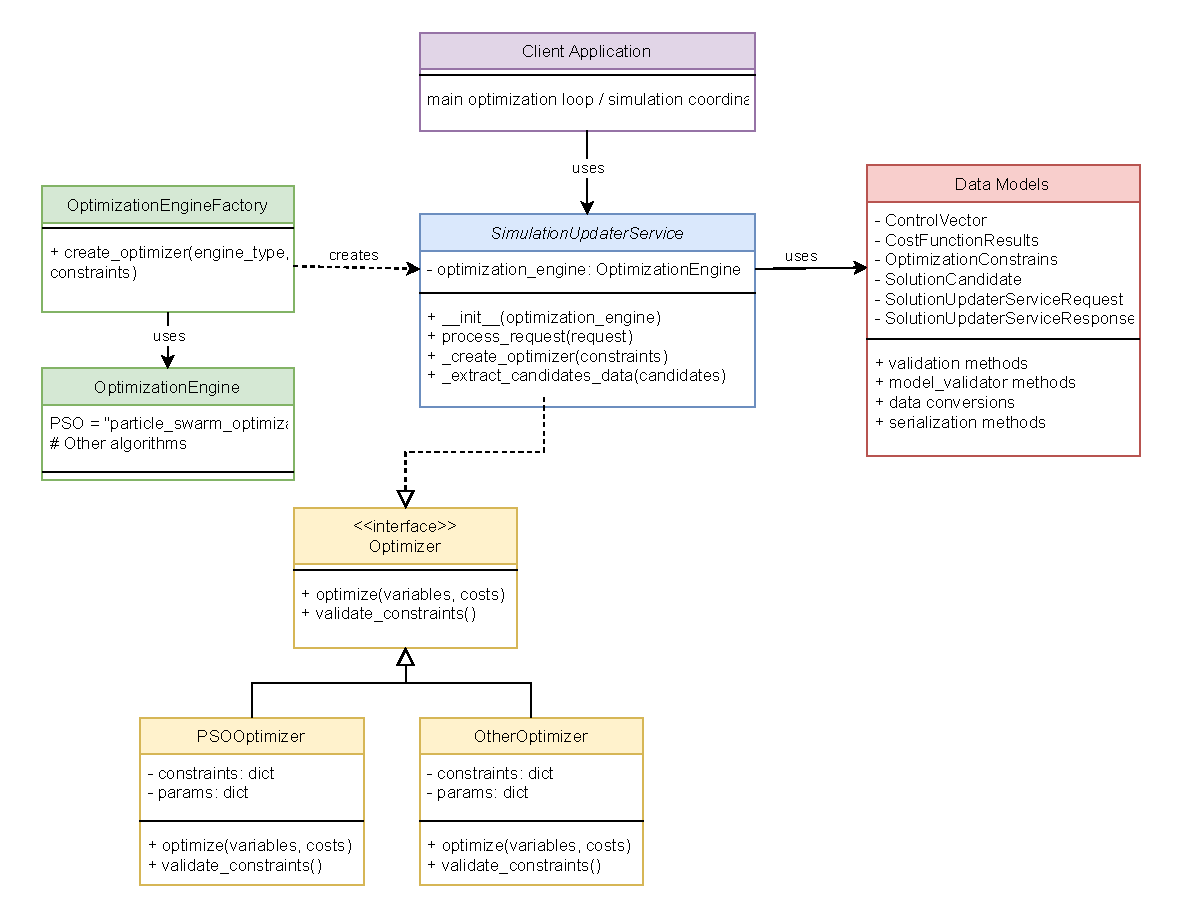
\includegraphics[width=1.0\textwidth]{content/images/SolutionUpdaterUML.pdf}
	\caption{Simulation updater service system UML}
	\label{fig:SolutionUpdaterServiceUML}
\end{figure}

\bigskip
\textbf{System Components}

The \texttt{SimulationUpdaterService} consists of several interconnected components that work together to provide optimization capabilities:

\begin{itemize}
\item \textbf{SimulationUpdaterService}

The main service class that exposes the public API and orchestrates the optimization process.

\textbf{Responsibilities:}
\begin{itemize}
	\item Provide a public interface for clients
	\item Coordinate the optimization workflow
	\item Manage the optimization loop
	\item Check convergence criteria
	\item Return processed results
\end{itemize}

\item \textbf{\_Mapper}

Internal component responsible for translating between domain-specific data structures and numerical representations suitable for optimization algorithms.

\textbf{Responsibilities:}
\begin{itemize}
	\item Convert control vectors to numpy arrays
	\item Convert optimization results back to domain objects
	\item Maintain mappings between domain and numerical representations
	\item Handle variable bounds and constraints
	\item Initialize mapping on first execution
\end{itemize}

\item \textbf{\_MapperState}

Maintains the state of mappings between control vectors, simulation results, and their numerical representations.

\textbf{Responsibilities:}
\begin{itemize}
	\item Store control vector mapping information
	\item Store results mapping information
	\item Track control vector dimensions
	\item Track results dimensions
	\item Store population size information
\end{itemize}

\item \textbf{\_SolutionUpdaterServiceLoopController}

Controls the execution of the optimization loop, tracking progress and termination conditions.

\textbf{Responsibilities:}
\begin{itemize}
	\item Track current generation number
	\item Enforce maximum generation limit
	\item Provide running state information
	\item Offer context manager for loop control
	\item Support early termination
\end{itemize}

\item \textbf{Optimization Engine}

Encapsulated component that implements the mathematical optimization algorithms.

\textbf{Responsibilities:}
\begin{itemize}
	\item Execute numerical optimization operations
	\item Apply optimization techniques to solution arrays
	\item Generate updated solutions based on fitness evaluations
	\item Handle constraints in the optimization process
\end{itemize}

\end{itemize}

\textbf{Public API}

The \texttt{SimulationUpdaterService} exposes a minimal yet powerful public API that provides access to its optimization capabilities. This section details each public method, its parameters, return values, and implementation details.

\begin{itemize}
	\item SimulationUpdaterService Constructor

	Initializes a new instance of the \texttt{SimulationUpdaterService} class. This constructor sets up the internal components required for the optimization process, including the mapper, optimization engine, and loop controller.

	\textbf{Implementation Details}

	The constructor performs the following initialization steps:
	\begin{itemize}
		\item Creates a new instance of the \texttt{\_Mapper} class for domain-numerical translation
		\item Initializes the optimization engine with default configuration
		\item Sets up a logger for diagnostic information
		\item Creates a \texttt{\_SolutionUpdaterServiceLoopController} instance to manage the optimization loop
	\end{itemize}

	\textbf{Error Handling}
	\begin{itemize}
		\item Any exceptions during initialization are allowed to propagate, as they indicate critical setup problems that should prevent service creation
		\item If dependencies are not available or incorrectly configured, appropriate import or initialization errors will be raised
	\end{itemize}

	\item \csignature{process\_request(self, request)}

	Processes an optimization request by iteratively updating the solution based on simulation results. This method represents the core functionality of the service, orchestrating the complete optimization workflow from initial population to converged solutions.

	\textbf{Implementation Details}

	The method implements a complete optimization step:
	\begin{enumerate}
		\item Validates the input request for required fields and data consistency
		\item Initializes the mapper with the domain-specific structure of control vectors and results
		\item Converts the domain objects to numerical arrays suitable for optimization
		\item Sets up the optimization loop with appropriate constraints and parameters
		\item Executes the optimization process for multiple generations until convergence or maximum generations
		\item Periodically checks for convergence based on defined criteria
		\item Translates the optimized numerical results back to domain-specific control vectors
		\item Prepares and returns a comprehensive response with the optimization results
	\end{enumerate}

	\textbf{Error Handling}
	\begin{itemize}
		\item \textbf{ValueError}: Raised if the request is missing required fields or contains inconsistent data
		\begin{itemize}
			\item Missing initial population or simulation results
			\item Mismatch between population size and results size
			\item Invalid configuration parameters (negative max generations, etc.)
		\end{itemize}

		\item \textbf{TypeError}: Raised if the data types in the request are incompatible with the optimization process
		\begin{itemize}
			\item Non-numeric values in control vectors or results
			\item Incompatible constraint formats
		\end{itemize}

		\item \textbf{RuntimeError}: Raised if the optimization process encounters an unrecoverable error
		\begin{itemize}
			\item Optimization algorithm failure
			\item Numerical stability issues
			\item Resource limitations
		\end{itemize}

		\item \textbf{Exception Handling}: The method includes comprehensive exception handling to:
		\begin{itemize}
			\item Log detailed diagnostic information
			\item Provide informative error messages
			\item Clean up resources in case of failures
			\item Convert low-level numerical exceptions to domain-appropriate exceptions
		\end{itemize}
	\end{itemize}

	\item \textbf{Loop controller}

	A property that provides access to the optimization loop controller. The loop controller exposes information about the optimization process state and provides control over the execution of the optimization loop:

	\begin{itemize}
		\item Maintains state about the current generation number
		\item Tracks whether the optimization loop is currently running
		\item Provides a context manager for the optimization loop execution
		\item Enforces maximum generation constraints
		\item Supports early termination of the optimization process
	\end{itemize}

	The controller is typically used internally by the \texttt{process\_request} method, but is exposed as a public property to allow advanced clients to access detailed state information or implement custom loop control if needed.

\end{itemize}

\textbf{Data Models Schema}

The \texttt{SimulationUpdaterService} uses a structured set of data models to represent optimization problems, solution candidates, and constraints. This section details the schemas of these models and their relationships.

\begin{lstlisting}[language=Python, caption={OptimizationEngine enumeration definition}]
	class OptimizationEngine(Enum):
	"""Enumeration of available optimization algorithms."""

	PSO = "particle_swarm_optimization"
	# Other algorithm types can be added here
\end{lstlisting}

\textbf{Description:}
The \texttt{OptimizationEngine} enumeration defines the available optimization algorithms that can be used by the service. Currently, it includes Particle Swarm Optimization (PSO), but the system is designed to be extensible with additional algorithms in the future.

\begin{lstlisting}[language=Python, caption={ControlVector model definition}]
	from pydantic import BaseModel, Field

	class ControlVector(BaseModel, extra="forbid"):
	"""Represents a collection of optimization variables."""

	items: Dict[str, float]
\end{lstlisting}

\textbf{Description:}
The \texttt{ControlVector} model represents the input parameters that control a simulation. Each item in the dictionary corresponds to a single optimization variable (e.g., "pressure", "temperature") with its associated value. The optimization process will aim to find optimal values for these variables.

\textbf{Validation Requirements:}
\begin{itemize}
	\item The items dictionary must not be empty
	\item All keys must be strings representing variable names
	\item All values must be floating-point numbers within valid numerical ranges
\end{itemize}

\begin{lstlisting}[language=Python, caption={CostFunctionResults model definition}]
	from pydantic import BaseModel, Field

	class CostFunctionResults(BaseModel, extra="forbid"):
	"""Stores the results of cost function calculations."""

	values: Dict[str, float]
\end{lstlisting}

\textbf{Description:}
The \texttt{CostFunctionResults} model stores the output metrics from simulation runs. Each item in the dictionary represents a cost function (e.g., "heat\_transfer", "flow\_rate") with its calculated value. These values are used to evaluate how good a particular solution is and guide the optimization process.

\textbf{Validation Requirements:}
\begin{itemize}
	\item The values dictionary must not be empty
	\item All keys must be strings representing cost function names
	\item All values must be floating-point numbers
\end{itemize}

\begin{lstlisting}[language=Python, caption={OptimizationConstrains model with validation logic}]
	from pydantic import BaseModel, Field, model_validator

	class OptimizationConstrains(BaseModel, extra="forbid"):
	"""Defines the constraints for the optimization variables."""

	boundaries: Dict[str, Tuple[float, float]]

	@model_validator(mode='after')
	def validate_lower_bound_is_less_than_upper_bound(self) -> 'OptimizationConstrains':
	"""Validates that lower bounds are less than upper bounds."""
		for var_name, (lower, upper) in self.boundaries.items():
			if lower >= upper:
				raise ValueError(
				f"Lower bound must be less than upper bound for {var_name}. "
				f"Got: lower={lower}, upper={upper}"
		)
	return self
\end{lstlisting}


\textbf{Description:}
The \texttt{OptimizationConstrains} model defines the valid ranges for optimization variables. Each entry in the boundaries dictionary maps a variable name to its allowed range as a tuple of (lower\_bound, upper\_bound). The optimization process will ensure that all solutions stay within these boundaries.

\textbf{Validation Requirements:}
\begin{itemize}
	\item For each variable, the lower bound must be strictly less than the upper bound
	\item All boundary values must be valid floating-point numbers
	\item Variable names in boundaries should match those used in ControlVector
\end{itemize}

\begin{lstlisting}[language=Python, caption={SolutionCandidate model definition}]
	from pydantic import BaseModel, Field

	class SolutionCandidate(BaseModel, extra="forbid"):
	"""Represents a complete solution with inputs and results."""

	control_vector: ControlVector
	cost_function_results: CostFunctionResults
\end{lstlisting}

\textbf{Description:}
The \texttt{SolutionCandidate} model represents a complete solution in the optimization process, pairing a specific set of input parameters with their resulting simulation outputs. Each candidate represents one point in the solution space, and the optimization process evaluates and compares candidates to find better solutions.

\textbf{Validation Requirements:}
\begin{itemize}
	\item Both control\_vector and cost\_function\_results must be provided
	\item The control\_vector must be a valid ControlVector instance
	\item The cost\_function\_results must be a valid CostFunctionResults instance
\end{itemize}

\begin{lstlisting}[language=Python, caption={SolutionUpdaterServiceRequest model with complex validation logic}]
	from pydantic import BaseModel, Field, model_validator
	from typing import List, Optional

	class SolutionUpdaterServiceRequest(BaseModel, extra="forbid"):
		"""The complete request for optimization."""

		solution_candidates: List[SolutionCandidate]
		optimization_constraints: Optional[OptimizationConstrains] = None

	@model_validator(mode='after')
	def validate_solution_candidates_contain_the_same_cost_functions(self) -> 'SolutionUpdaterServiceRequest':
		"""Validates that all solution candidates use the same set of cost functions."""
		if not self.solution_candidates:
			return self

		reference_candidate = self.solution_candidates[0]
		reference_cost_functions = set(reference_candidate.cost_function_results.values.keys())

		for idx, candidate in enumerate(self.solution_candidates[1:], start=1):
			candidate_cost_functions = set(candidate.cost_function_results.values.keys())
			if reference_cost_functions != candidate_cost_functions:
				raise ValueError(
					f"All solution candidates must contain the same cost functions. "
					f"Mismatch at candidate {idx}. "
					f"Expected: {reference_cost_functions}, "
					f"Got: {candidate_cost_functions}"
				)
		return self

	@model_validator(mode='after')
	def validate_solution_candidates_contain_the_same_optimization_variables(self) -> 'SolutionUpdaterServiceRequest':
		"""Validates that all solution candidates use the same set of optimization variables."""
		if not self.solution_candidates:
			return self

		reference_candidate = self.solution_candidates[0]
		reference_variables = set(reference_candidate.control_vector.items.keys())

		for idx, candidate in enumerate(self.solution_candidates[1:], start=1):
			candidate_variables = set(candidate.control_vector.items.keys())
			if reference_variables != candidate_variables:
				raise ValueError(
					f"All solution candidates must contain the same optimization variables. "
					f"Mismatch at candidate {idx}. "
					f"Expected: {reference_variables}, "
					f"Got: {candidate_variables}"
				)
		return self

	@model_validator(mode='after')
	def validate_optimization_boundaries_contain_the_same_optimization_variables(self) -> 'SolutionUpdaterServiceRequest':
		"""Validates that optimization boundaries match the variables used in solutions."""
		if not self.solution_candidates or not self.optimization_constraints:
			return self

		reference_candidate = self.solution_candidates[0]
		reference_variables = set(reference_candidate.control_vector.items.keys())
		boundary_variables = set(self.optimization_constraints.boundaries.keys())

		if reference_variables != boundary_variables:
			raise ValueError(
				f"Optimization boundaries must contain the same variables as solution candidates. "
				f"Solution variables: {reference_variables}, "
				f"Boundary variables: {boundary_variables}"
			)
			return self

	@model_validator(mode='after')
	def reorder_solution_candidates_optimization_variables_and_cost_functions(self) -> 'SolutionUpdaterServiceRequest':
		"""Reorders variables and cost functions for consistent processing."""
		# Implementation handles consistency of ordering across solution candidates
		return self
\end{lstlisting}

\textbf{Description:}
The \texttt{SolutionUpdaterServiceRequest} model represents a complete request to the optimization service. It contains the initial population of solution candidates and optional constraints. The service processes this request to generate an optimized set of solutions.

The model includes several validation methods to ensure consistency across the solution candidates:
\begin{itemize}
	\item Ensures all candidates use the same cost functions
	\item Ensures all candidates use the same optimization variables
	\item Verifies that optimization boundaries match the variables used
	\item Reorders variables and cost functions for consistent processing
\end{itemize}

\textbf{Validation Requirements:}
\begin{itemize}
	\item Must contain at least one solution candidate
	\item All solution candidates must use the same set of cost function names
	\item All solution candidates must use the same set of optimization variable names
	\item If constraints are provided, they must cover the same variable names
\end{itemize}







\bigskip
\textbf{Detailed Workflow}
The optimization process within the \texttt{SimulationUpdaterService} follows a systematic workflow that translates domain-specific inputs into optimized outputs through several processing stages.

\begin{enumerate}

\item Initialization Phase

\begin{enumerate}
	\item \textbf{Request Validation}: The service validates the incoming request to ensure it contains the required data.

	\item \textbf{Mapper Initialization}: On first execution, the mapper analyzes the structure of control vectors and results to create appropriate mappings.

	\item \textbf{State Preparation}: The service initializes the optimization state, including:
	\begin{itemize}
		\item Population arrays
		\item Results arrays
		\item Constraint definitions
		\item Variable bounds
		\item Generation counters
	\end{itemize}

	\item \textbf{Engine Configuration}: The optimization engine is configured with appropriate parameters for the specific problem.
\end{enumerate}

\item Optimization Step

The main optimization step executes the following steps for each generation:

\begin{enumerate}
	\item \textbf{Population Conversion}: Control vectors are converted to numerical arrays using the mapper.

	\item \textbf{Fitness Evaluation}: The fitness of each solution is calculated based on simulation results.

	\item \textbf{Selection}: The most promising individuals are selected for producing the next generation.

	\item \textbf{Variation Operations}: The optimization engine applies:
	\begin{itemize}
		\item Crossover between selected individuals
		\item Mutation to maintain diversity
		\item Constraint handling to ensure valid solutions
	\end{itemize}

	\item \textbf{Population Update}: The new generation replaces the previous one.

	\item \textbf{Convergence Check}: The service evaluates whether the optimization has converged using:
	\begin{itemize}
		\item Change in objective function values
		\item Population diversity metrics
		\item Constraint satisfaction levels
		\item Stability of the best solution
	\end{itemize}

	\item \textbf{Loop Control}: The controller updates generation counters and checks for termination conditions.
\end{enumerate}

\item Finalization Phase

After the optimization step completes (either through convergence or reaching maximum generations):

\begin{enumerate}
	\item \textbf{Result Translation}: The final numerical solutions are converted back to domain-specific control vectors.

	\item \textbf{Metrics Compilation}: Convergence metrics and optimization statistics are compiled.

	\item \textbf{Response Preparation}: A structured response is created containing:
	\begin{itemize}
		\item Optimized control vectors
		\item Convergence metrics and history
		\item Termination reason
		\item Generation statistics
	\end{itemize}

	\item \textbf{Resource Cleanup}: Any temporary resources used during optimization are released.
\end{enumerate}

\end{enumerate}

\subsection{Problem dispatcher service}


\end{document}
